%!TEX root = umthsmpl.tex
\chapter{Difficulty Estimation}
\label{difficulty-estimation}

\section{Problem Statement}
\section{Preliminary Work}
\subsection{Analysis of Difficulty Estimation}
\subsection{Alternative Estimation}
\section{Proposed Work}

%\paragraph*{Overview}

%\begin{equation}
%\arg\max_\mathbf{s} p(\mathbf{s}|u).
%\end{equation}
%
%\begin{figure}\begin{center}
%		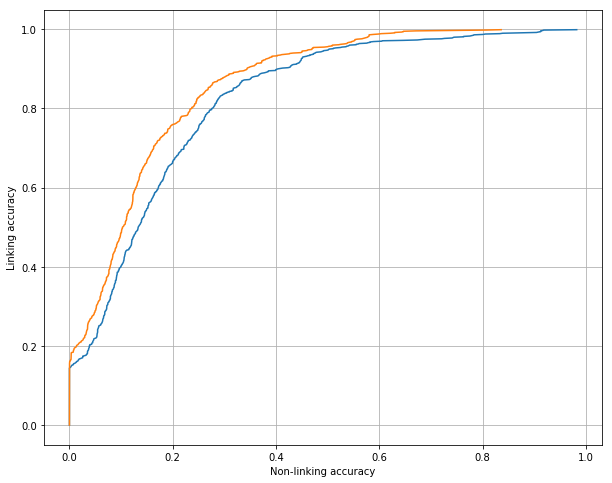
\includegraphics[width=0.7\textwidth]{graphics/linking2}
%		\caption{The $x$-axis represents accuracy of identifying a set of traces unlinked, and the $y$-axis represents the accuracy of the same set linked based on Equation~\ref{eq:link3}. Red is a link before, and blue is a link after.
%		\label{fig:linkcdf}}
%\end{center}\end{figure}